\documentclass[../main.tex]{subfiles}
\graphicspath{{\subfix{../IMAGES/}}}

\begin{document}
\localtableofcontents

\subsection{Electromechanical energy conversion}
The winding voltage is linked to the winding current and flux linkage by : $\Vec{v} = R \Vec{i} + \frac{d\vec{\phi}}{dt}$.\\
On the mechanical side : $J \frac{d \omega}{dt} + F(\omega) \omega = T_{em}-T_m$, $F$ the friction coefficient. \\
States variables are fluxes, rotor angle, rotor angular speed. System inputs are voltages and loading torque. System outputs are currents and electromagnetic torque.\\
By conversion of energy : $P_{in} = P_{out} + \frac{dW}{dt} + P_{loss}$, with $P_{in} = \sum i_k \frac{d\phi_k}{dt} = \vec{i}^T \frac{d\vec{\phi}}{dt}$, $P_{out} = T_{em} \omega$. Neglect internal losses. Then : $\frac{dW}{dt} = \frac{dW_{em}}{dt} = \sum \frac{\partial W_{em}}{\partial \phi_k}\frac{d\phi_k}{dt}  + \frac{\partial W_{em}}{\partial \theta} \frac{d\theta}{dt}$, $i_k = \frac{\partial W_{em}}{\partial t}$ and $T_{em} = -\frac{\partial W_{em}}{\partial \theta}$.\\
Let $W'_{em} = \vec{i}^T \vec{\phi}-W_{em}$. Then : $\phi_k = \frac{\partial W'_{em}}{\partial i_k}$ and $T_{em} = \frac{\partial W'_{em}}{\partial \theta}$.\\

Energy : $W_{em} = \iiint w_{em} dV$, $w_{em} = \int \vec{H}(\vec{B}) \cdot d\vec{B} = \frac{1}{2}\mu H^2$.\\
Coenergy : $W'_{em} = \iiint w'_{em} dV$, $w'_{em} = \int \vec{B}(\vec{H})\cdot d\vec{H} = \frac{1}{2} \frac{B^2}{\mu}$.\\

Materials in electric machines can be : dielectric (insulating), conductor, soft ferromagnetic, hard ferromagnetic (permanent magnet). Then : \begin{equation}
    \vec{B} = \mu \vec{H} + \vec{B}_{PM}
\end{equation}

\warning Energy and coenergy densities are equal in absence of permanent magnetization. Different in presence of permanent magnetization. \\

Flux linkages are found from the currents : $\phi_m = \frac{\partial W'_{em}}{\partial i_m} = W_{em,m}^{'(1)}(\theta) + \sum_{k2=1}^n[2W_{em,m,k2}^{'(2)}(\theta) i_{k2}] = \psi_{PM,m} (\theta)  + \sum_{k2=1}^n[L_{m,k2}(\theta) i_{k2}]$.\\
The total flux linkage is then : $\phi = \psi_{PM}(\theta) + L(\theta) i$. Then : $v = Ri + \omega[\frac{\partial \psi_{PM}}{\partial \theta} + \frac{\partial L}{\partial \theta} i]+ L(\theta) \frac{di}{dt}$.\\
The electromagnetic torque is then : \begin{equation}
    \begin{gathered}
        T_{em} = \frac{\partial W_{em}^{'(0)}}{\partial \theta} + \frac{\partial \psi_{PM}^T}{\partial\theta} i + \frac{1}{2}i^T \frac{\partial L}{\partial \theta}i\\
        \text{Torque = magnets only related torque + interaction currents/magnets + interaction currents/magnets.}
    \end{gathered}
\end{equation}

\warning For a two-winding machine only the stator-rotor inductance are variable : $T_{em} = \frac{1}{2}i^T \frac{\partial L}{\partial \theta}i$. The condition for non-zero average torque generation is : $\omega_s \pm \omega_r \pm p\omega_m = 0$.\\

\subsection{DC machine modeling}
Both stator and rotor electrical access terminals are supplied by DC current (can be with AC current if universal motor).\\
Types of excitation : separately excited DC machines (used for variable speed), series connected (universal motor, torque maximum at zero speed, used for traction machines), parallel connected (mainly for generator), compound (series and parallel). \\
If stator winding : excitation flux can be controlled, if permanent magnets, it cannot.\\

During commutation, commutator segments are short-circuited. Change of current direction happens in those conductors that are sc. Sc current is limited only by the impedance of the turn. To reduce magnetic induction in the neutral zone (zone without poles in the stator), DC machines can have compensation windings/auxiliary poles winding.\\

Magnetic axes of rotor and stator are perpendicular by machine design. On the direct axis : corresponds to the excitation flux (determined by the position of main poles), quadrature axis : corresponds to the armature reaction. The stator has three fluxes $\phi_f, \phi_{CW}, \phi_{AP}$ creating a resulting stator flux $\phi_s$. The rotor has one flux. Resultant flux along the direct axis is $\phi_f$.\\

Excitation flux : $\phi_f = SB_f = \mu_0 \frac{LW N_fI_f}{2\delta}$, with $\delta$ the air-gap length, $L$ the axial length and $W$ the width. 
\begin{figure}[hbt!]
    \centering
    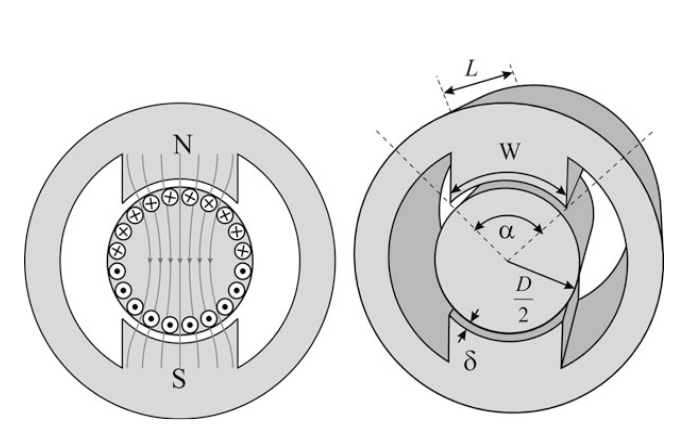
\includegraphics[width=0.5\linewidth]{IMAGES/Indus_el/Screenshot from 2025-03-03 16-23-35.png}
\end{figure}

The magnetic resistance along the excitation path : $R_\mu = \frac{F_f}{\phi_f} = \frac{2\delta}{\mu_0 LW}$. The inductance of the excitation winding : $L_f = \frac{\psi_f}{I_f} = \frac{N_f^2}{R_\mu}$.\\

\textbf{The EMF} is : $E = \vec{l} \cdot \vec{E_{ind}} = \vec{l} \cdot (\vec{v} \times \vec{B})$. In each of the conductors : $E_k = \pm r\cdot \omega_m \cdot B_f \cdot l$. Then, the \textbf{total induced emf} in the rotor winding : $E_a = (\frac{N_RW}{2\pi r}) B_f l r \omega_m = k_e \phi_f \omega_m$, $k_e$ the emf coefficient.\\

Each conductors contributes to the electromagnetic torque : $T_{em,k} = \frac{i_a}{2} l B_f r$ ($\frac{i_a}{2}$ as only half of the armature current flows in one conductor). The \textbf{total EMT} : $T_{em} = 2(N_R \frac{W}{2\pi r}) \frac{i_a}{2} l B_f r = k_m \phi_f i_a$. \\

For the excitation : $u_f = R_fi_f + L_f \frac{di_f}{dt}$, the flux is proportional to the excitation current : $\phi_f = \frac{L_f}{N_f} i_f$.\\
For the rotor (armature) : $u_a = R_ai_a + L_a \frac{di_a}{dt} + E_a = R_ai_a + L_a \frac{di_a}{dt} + k_e \phi_f \omega_m$.\\

\warning The EMF and torque constant are the same (conservation of energy) : $k_m=k_e$.\\

In steady state : $U_f = R_f I_f$, $U_a = R_aI_a + k_e \phi_f \Omega_m$. When no load : $\Omega_0 = \frac{U_m}{k_e \phi_f}$ (as $I_a = 0\Rightarrow T=0$). Any increase of load torque increases armature current. \\

\warning Let $S$ be the stiffness/slope of the mechanical characteristic (here : $S = \frac{k_mk_e\phi_f^2}{R_a}$) with $T_{em} = T_0 - S_{em}\Omega_m$ and $T_m = T_0-S_m \Omega_m$. The system is considered stable if : $S_m-S_{em} <0$ as a small change in the speed gradually decreases and bring the system back to original point.\\
The change of machine temperature is : $P_\gamma = \frac{\Delta \theta}{R_T} + C_T \frac{d\Delta \theta}{d_t}$ with a thermal time constant : $\tau = R_T C_T$.\\


\subsection{DC machine control}

\begin{figure}
    \centering
    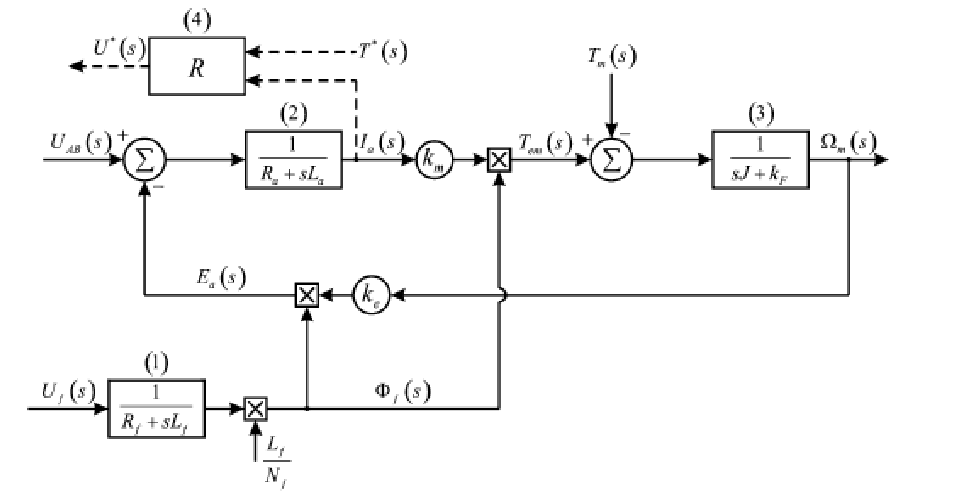
\includegraphics[width=0.5\linewidth]{IMAGES/Indus_el/Screenshot from 2025-03-03 16-47-33.png}
    \caption{Block diagram of the DC machine model}
\end{figure}

Inputs are : excitation and armature voltage. State variables are armature current, excitation current and rotor speed. Outputs are armature current, excitation flux, electromagnetic torque and rotor speed.\\
Power of supply : excitation ($P_f = R_fI_f^2$), armature winding ($P_a = R_aI_a^2 + E_aI_a$). Mechanical power at the output : $P_m = T_m\omega_m = P_c-P_{fe}-P_F = E_aI_a - P_{fe}-P_F$.\\

A full bridge converter can serve all four quadrants. PWM is required to provide average output voltage. A bipolar PWM thecnique (applied discrete armature voltage is either E or -E) has an average voltage of : $U_{av} = \frac{2t_{ON}-T_{PWM}}{T_{PWM}} E = (2m-1) E$.\\
With a unipolar PWM technique, the applied discrete armature voltage is either E, 0, -E : $U_{av} = \frac{t_{on}}{T_{PWM}} E = \pm dE$.\\
Transfer function of the armature winding : $W(s) = \frac{I_a}{U_a-E_a} = \frac{1}{sL_a+R_a}$. At high frequencies : $W(s) \simeq \frac{1}{sL_a}$.\\
The current ripple is then (bipolar modulation) : $\Delta I_a = \frac{T_{PWM}E}{L_a} (m-m^2)$ (highest current ripple at $m=0.5$ : $\Delta I_{a,max} = \frac{T_{PWM} E}{4L_a}$).\\

Torque could be controlled by changing the flux or armature current but changing flux is slow.\\
A PI controller can be used to control the armature current $i_a$. \\
\begin{figure}[hbt!]
    \centering
    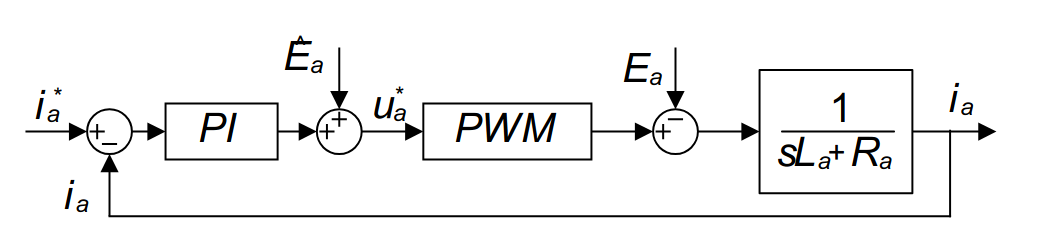
\includegraphics[width=0.5\linewidth]{IMAGES/Indus_el/Screenshot from 2025-03-03 17-12-49.png}
\end{figure}

\warning The PWM controlled converter can be treated as a simple delay block $T_d = 1.5T_s$.\\

\begin{figure}[hbt!]
    \centering
    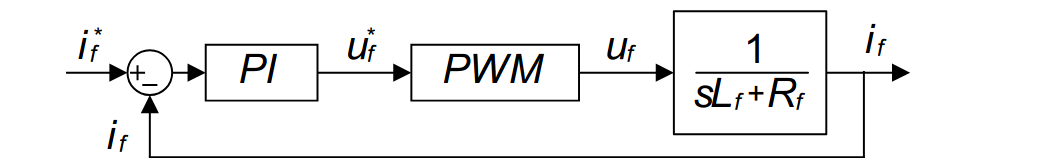
\includegraphics[width=0.5\linewidth]{IMAGES/Indus_el/Screenshot from 2025-03-03 17-14-14.png}
\end{figure}

\begin{figure}[hbt!]
    \centering
    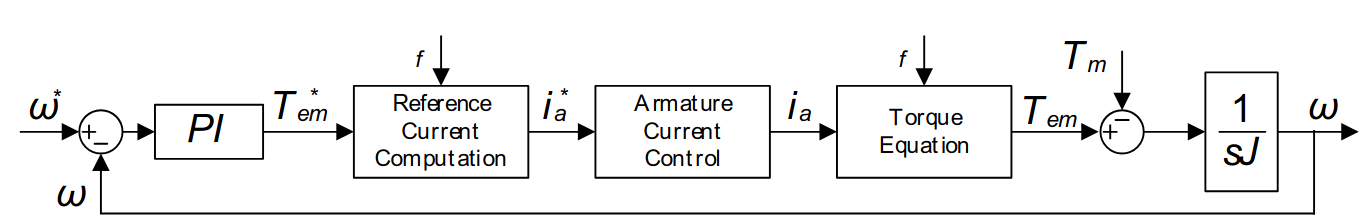
\includegraphics[width=0.5\linewidth]{IMAGES/Indus_el/Screenshot from 2025-03-03 17-15-19.png}
\end{figure}

The armature voltage needs to compensate higher EMFs at higher speed : $U_a \simeq E_a = k_e \phi_f \omega_m$. The rated speed is : $\omega_{m,n}= \frac{U_{a,n}}{k_e \phi_{f,n}}$, above the rated speed, the control strategy should be changed : \textbf{Field weakening}. The flux should decrease in order to keep the EMF constant $E_a$ which leads to a reduction of torque but a constant power. 



\subsection{Sensors}

Types : tachogenerators (provide rotational speed sensing), encoders (incremental, absolute), electromagnetic resolvers (provide measurements on both speed and position).\\

\subsubsection{Tachogenerator}
Generates output voltage proportional to the shaft speed : $E_a = k_e\phi_f \omega_m$. Could be done with a permanent magnet AC generators. \\

\subsubsection{Encoders}
\quad \underline{Incremental : } \\
LED is pulsed by the rotating disk slots. It crosses a mask and reaches the photo-detector. In general, it has two channels denoted A and B that generates many pulses per revolution. Channels are arranged in quadrature such as one can extract angular speed and direction. We can also have a z channel that generates a single reference pulse per revolution.\\
For each period of the channel A square wave, four pulse edges can be counted, if pulses in channel B follow the pulses in channel A : positive direction. \\

For example : consider a double-channel IE with 1000 slots per track. This yields a number of $N_{eT} = 4000$ edges/rev. Rotational speed is periodically calculated within a period of time $T_c \: (1ms)$. \\
At \textbf{high speed}, we count the number of edges $N_c$. The speed of the machine is then : \begin{equation}
    n_{mach} = 60 \frac{N_c}{T_c} \frac{1}{N_{eT}} \: [RPM]
\end{equation}

At \textbf{low speed}, one measures the time of every pulses. Time elapsed between two edges : $\Delta T$, the interval between two edges is linked to the distance between two slots : $r_{min} = \frac{1}{N_{eT}}$, then : \begin{equation}
    n_{mach} = 60 \frac{1}{N_{eT}} \frac{1}{\Delta T} \: [RPM]
\end{equation}
\warning This method is only to be used at low speed.\\

\quad \underline{Absolute :}\\
It is a position measurement device. No reference is needed. Disk has several concentric tracks each of them with independent light source. Works as binary (many tracks : around 12).\\
For N tracks, the number of increments/rev is : $n_i = 2^N$, the angular value of each increment : $\delta = 360^\circ/2^N$. \warning Gray code are used (only one bit changes at a time to reduce risk of error).\\

\subsubsection{Electromagnetic resolvers}
Analog transducer which operated as a rotary transformer. Based on the fact that induced EMF between two coils depends on their mutual displacement. Consists of a stator and a rotor. Stator contains three windings (one exciter mounted on the axis of the resolver, two secondary windings shifted by $90^\circ$ : sine and cosine windings). Rotor contains the secondary of the rotary transformer, primary winding of the resolver. $\theta = \arctan \frac{V_s}{V_c}$.\\
They offer infinite theoretical resolution (as they are analog devices).\\

\subsubsection{Hall effect}
It can be used to measure the magnetic flux density field in specific point of space. Open loop solutions are affected by limited bandwidth and gain drift with temperature. \\
Closed loop : the current to be measured $I_p$ creates a magnetic flux which crosses the Hall effect sensor in the core airgap. The voltage produced by the hall device is used to drive the secondary current $I_s$. This current counterbalances the primary flux such that the induced voltage is 0. \\

To measure voltage : same idea but instead of having the conductor in the middle of the coil, it is applied to the primary coil. 

\subsubsection{Resistive divider}
The shunt is comprised of two series high-resistance resistors. The upper resistors are in the range of $M\Omega$ while the bottom $k\Omega$. A shunt is a low-resistance resistor whose voltage drop provides an image of current flowing. For measuring AC current : either inline or low-side (under the 3phase inverter, cheaper, easier).\\
For low-side shunt current sensor the sampling must be triggered when the low-side device is in ON state. You can even remove one sensor (if system is balanced). To make it even more low cost : use only one sensor.\\

\begin{figure}[hbt!]
    \centering
    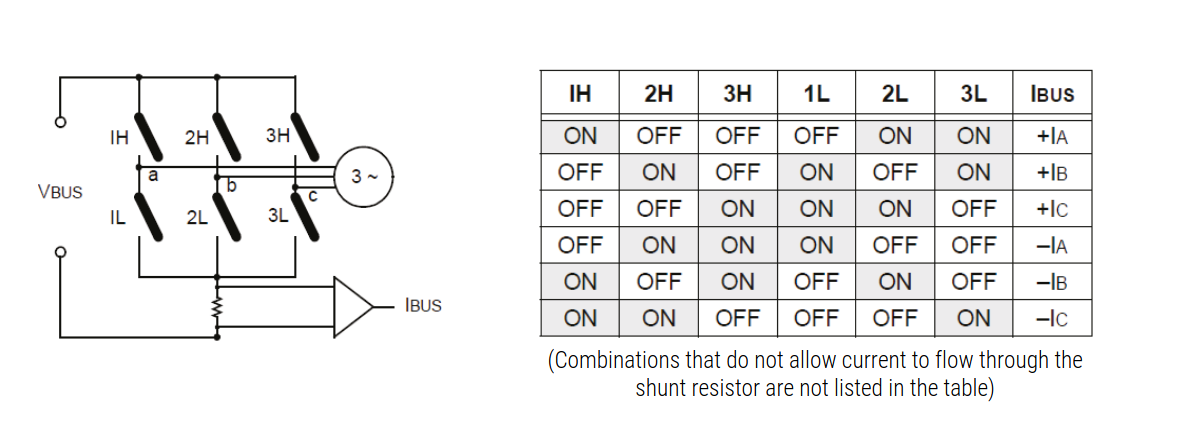
\includegraphics[width=0.8\linewidth]{IMAGES/Indus_el/Screenshot from 2025-03-10 17-36-37.png}
\end{figure}

\warning In case of the use of only one sensor : modulation pattern must be adapted.


\subsection{AC machine windings}
Magnetic circuits of the stator and rotor are made of iron sheets. \\
The head connections do not participate in the EM energy conversion (analysis only on the active length). It is sufficient to analyse a single 2D slice of the machine, the magnetic flux and magnetomotive force (MMF) are only present in the air-gap. Only radial component of the magnetic flux is present. \\

The MMF at position $\alpha$ : $F(\alpha) = \int H t dl = H(\alpha) \delta t$, with $\delta t$ the field line length and $H(\alpha)$ the magnetic field at angle $\alpha$. This generates a square wave. The peak value is : $F_{max} = \frac{Z_f I}{4}$ while the magnitude of the fundamental component is : $F_1 = \frac{Z_f I}{\pi}$. \\
In a distributed winding, multiple coils are located in different slots; their MMF waveforms can be composed together. A staircase MMF waveform is generated. The magnitude of the fundamental component is lower than in the concentrated case : $F_1 = \frac{Z_fI}{\pi} \frac{\sin(q \beta/2)}{q\sin( \beta/2)} = \frac{Z_fI}{\pi} K_d$.\\
In many cases, conductors of a coil are not positioned diametrically but at an angle less than $180^\circ$. The winding can be divided in multiple layers. It causes the decrease of magnitude : $F_{1tot} = F_{1,layer} K_r$. A winding can be identified by an equivalent Number of Turns that generates only the sinusoidal component of the MMF : $F_{1tot} = (K_a \frac{Z_f}{\pi}) I$.\\
The number of identical repetitions defines the pole pairs of the winding $P_p$.An electrical angle is defined as a reference covering only $360^\circ/P_p$ mechanical angles. Then : $\alpha_e = P_p\alpha$, $\beta_e = P_p\beta$, $F_{1tot} = K_a \frac{Z_f}{P_p \pi}$, $K_a = K_rK_d$.\\
The magnetic flux density field in the air-gap is : $B(\alpha) = \mu_0 H_{\alpha}$.\\

$N' = K_a \frac{Z_f}{\pi P_p}$.

All phases are : $F_{s,a} (\alpha_e) = N_s' i_{s,a} \cos(\alpha_e+\varphi)$. The total is then : $F_s(\alpha_e) = \Re(\frac{3}{2} N_s' \underline{i_s} e^{-j\alpha_e})$.\\
Clarke's transform : $\begin{pmatrix}
    i_{s,\alpha}\\ i_{s,\beta}
\end{pmatrix} = \frac{2}{3} \begin{pmatrix}
    1 & -1/2 & -1/2\\ 0 & \sqrt{3}/2 & -\sqrt{3}/2
\end{pmatrix} \begin{pmatrix}
    i_{s,a}\\ i_{s,b}\\ i_{s,c}
\end{pmatrix}$.\\

For an m-phase system : $\underline{i} = i_\alpha + j i_\beta = \frac{2}{m} \sum i_k e^{j\alpha_k}$. Normally, only the odd-order harmonics are present for symmetric windings. The angle w.r.t the rotor reference is linked to the electrical reference via the rotor electrical position : $\theta_e = P_p \theta_m$ such that : $\alpha_e = \alpha_e^r + \theta_e$.\\

Consider the case where only two windings are present. The EM energy stored in the machine is : $W_{em} = \frac{1}{2} L_1 i^2 + \frac{1}{2}L_2 i^2 + L_m i_1 i_2$. The energy is stored only in the air-gap and the field is only radial : $L_1 = \frac{N_1^{'2}}{R_{m,eq}}$, $L_2 = \frac{N_2^{'2}}{R_{m,eq}}$, $L_m = \frac{N_1' N_2'}{R_{m,eq}} \cos(\alpha_1-\alpha_2)$, $R_{m,eq} = \frac{1}{\mu_0} \frac{\delta_0}{S_{coil}}$, $S_{coil} = lr\pi$.

\subsection{Induction machine modeling}
Stator can either be squirrel cage or wound rotor (with slip rings and called doubly-fed induction machine). $\omega_s = \omega_M + \omega_R$ with $\omega_s = 50Hz$ and $\omega_R$ can be controlled if doubly fed.\\
Both stator and rotor have to be laminated. Bars in the stator are often tilted (skewing) to reduce cogging torque effect (such as in a stepper motor). \\

\subsubsection{Control in the abc frame}
Assumptions : air-gap MMF is perfectly sinusoidal, stator has a symmetrical 3-phase winding, rotor is perfectly short-circuited. \\

Rotor voltages are zero, currents and fluxes are non-zero. In vectorial mode : $v_s = R_s i_s + \frac{d\phi_s}{dt}$ and $v_r = R_r i_r + \frac{d\phi_r}{dt}$. With $\phi = Li = L_l i + L_mi$, the inductance matrix can be decomposed into leakage inductance matrix and mutual inductance. The $L_l$ considers fluxes that do not go in the air-gap; the windings are decoupled (diagonal 6x6). The $L_m$ considers fluxes that go in the air-gap; all windings are coupled. In general : $L_m = \frac{N_1'N_2'}{R_{m,eq}} \cos(\alpha_1-\alpha_2)$.\\
Then : $\phi_s = L_{l,s} i_s + L_{s,s} i_s+ L_{s,r}(\theta_e) i_r$ and $\phi_r = L_{l,r} i_r + L_{r,r} i_r+ L_{s,r}^T(\theta_e) i_s$. With $L_{s,s} = L_{m,s} \begin{pmatrix}
    1&-1/2&-1/2\\-1/2&1&-1/2\\-1/2&-1/2&1
\end{pmatrix}$ ($L_{m,s} = \frac{N_s^{'2}}{R_{m,eq}}$), $L_{r,r} = L_{m,r} \begin{pmatrix}
    1&-1/2&-1/2\\-1/2&1&-1/2\\-1/2&-1/2&1
\end{pmatrix}$ ($L_{m,s} = \frac{N_s^{'2}}{R_{m,eq}}$).

Also $L_{s,r} = L_{m,sr} \begin{pmatrix}
    \cos(\theta_e) & \cos(\theta_e+120^\circ) & \cos(\theta_e+240^\circ)\\ \cos(\theta_e-120^\circ) & \cos(\theta_e) & \cos(\theta_e+120^\circ)\\ \cos(\theta_e-240^\circ) & \cos(\theta_e-120^\circ) & \cos(\theta_e)\\
\end{pmatrix}$ ($L_{m,sr} = \frac{N_s^{'} N_r'}{R_{m,eq}}$).\\

Also : $T_{em} = \frac{1}{2}i^T \frac{\partial L}{\partial \theta_m} i = P_p i_s^T \frac{\partial L_{s,r}}{\partial \theta_e} i_r$. $\theta_e = P_p \theta_m$.\\

\subsubsection{Space vector modeling}
Apply clarke's transformation : $\underline{x} = x_\alpha + jx_\beta = \frac{2}{3}(x_a + x_b e^{j2\pi/3} + x_c e^{j4\pi/3})$ (amplitude invariant definition). \warning Zero-sequence components can almost always be neglected.\\

$\begin{pmatrix}
    \phi_{s,\alpha}\\ \phi_{s,\beta} \\ \phi_{r,\alpha} \\ \phi_{r,\beta}\\
\end{pmatrix} = \begin{pmatrix}
    L_s & 0 & L_m \cos(\theta_e) & -L_m \sin(\theta_e)\\ 0 & L_s & L_m\sin \theta_e & L_m \cos \theta_e\\ L_m \cos \theta_e & L_m \sin \theta_e & L_r & 0\\ -L_m \sin \theta_e & L_m \cos \theta_e & 0 &L_r
\end{pmatrix} \begin{pmatrix}
     i_{s,\alpha}\\ i_{s,\beta} \\ i_{r,\alpha} \\ i_{r,\beta}\\
\end{pmatrix}$. The torque also becomes : $T_{em} = \frac{3}{2} P_p L_m [(i_{r,\alpha} i_{s,\beta} - i_{r,\beta} i_{s,\alpha})\cos\theta_e - (i_{r,\alpha} i_{s,\alpha} + i_{r,\beta} i_{s,\beta})\sin\theta_e]$. Inductances also become : $L_s= L_{l,s} + 3/2 L_{m,s}$, $L_r = L_{l,r} + 3/2 L_{m,r}$, $L_m = 3/2 L_{m,r}$.\\

\subsubsection{Common reference frame, dq control}
The space vector formalism uses two distinct reference frames for stator and rotor vectors. It is convenient to use a common reference frame : Parke transform.\\
To transform stator variables : $\theta_{park} = \theta_d$ and to transform rotor variables : $\theta_{park} = \theta_d- \theta_e$.\\
\warning The common reference frame can be chosen arbitrarily. \\

Then, $\begin{cases}
    v_{s,d} = R_s i_{s,d} + \frac{d\phi_{s,d}}{dt} - \omega_d \phi_{s,q}\\
    v_{s,q} = R_s i_{s,q} + \frac{d\phi_{s,d}}{dt} + \omega_d \phi_{s,d}
\end{cases}$ and $\begin{cases}
    0 = v_{r,d} = R_r i_{r,d} + \frac{d\phi_{r,d}}{dt} - (\omega_d - \omega_e) \phi_{r,d}\\
    0 = v_{r,q} = R_r i_{r,q} + \frac{d\phi_{r,q}}{dt} + (\omega_d - \omega_e) \phi_{r,q}\\
\end{cases}$.\\
$\begin{pmatrix}
    \phi_{s,d}\\ \phi_{s,q} \\ \phi_{r,d} \\ \phi_{r,q}\\
\end{pmatrix} = \begin{pmatrix}
    L_s & 0&L_m&0\\0&L_s&0&L_m\\L_m&0&L_r&0\\0&L_m&0&L_r
\end{pmatrix} \begin{pmatrix}
    i_{s,d}\\ i_{s,q} \\ i_{r,d} \\ i_{r,q}\\
\end{pmatrix}$. The torque is also : $T_{em} = \frac{3}{2} P_p L_m (i_{s,q} i_{r,d} - i_{s,d}i_{r,q})$.\\
\warning In this method, inductance matrix coefficients are all constant and the torque does not depend on rotor position.\\

\subsubsection{Scalar control}
Consider the stator reference frame ($\omega_d = 0$). In ss operation, all the electric variables are rotating vectors at $\omega_s$. The slip is defined as : $s = \frac{w_{slip}}{w_s} = 1-\frac{w_e}{w_s}$.\\

\begin{figure}[hbt!]
    \centering
    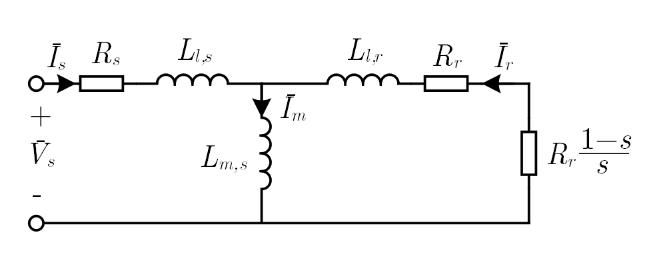
\includegraphics[width=0.5\linewidth]{IMAGES/Indus_el/Screenshot from 2025-04-07 16-23-23.png}
\end{figure}

The rotor resistance is displayed as : $R_r$ (joule losses). The equivalent mechanical resistance : $R_r \frac{1-s}{s}$ (power conversion el-mech).\\
Then : $P_{em} = \frac{3}{2} R_r \frac{1-s}{s} I_r^2$, $T_{em} = \frac{3}{2} \frac{P_r R_r}{sw_s} I_r^2$ with : $-I_r = \frac{V_s}{Z_s + Z_r + (Z_sZ_r/Z_m)}$, $Z_s = R_s+jw_s L_{l,s}$, $R_r/s + jw_s L_{l,r}$, $Z_m = jw_s L_{m,s}$.\\
Then : \begin{equation}
    T_{em} = \frac{3}{2} \frac{P_p R_r}{sw_s} \frac{V_s^2}{(R_s+R_r/s)^2 + w_s^2(L_{l,s} + L_{l,r})^2}
\end{equation}

\begin{figure}[hbt!]
    \centering
    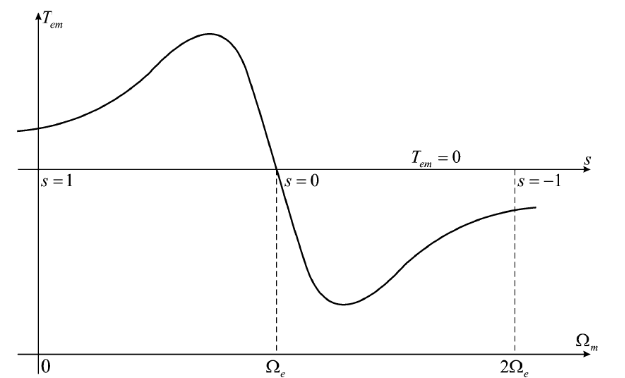
\includegraphics[width=0.5\linewidth]{IMAGES/Indus_el/Screenshot from 2025-04-07 16-28-49.png}
\end{figure}

For small slip : $T_{em} = \frac{3}{2} \frac{P_p}{R_r} \frac{V_s^2}{w_s^2} w_{slip}$, $I_r^2 \simeq I_s^2 \simeq \frac{V_s^2}{(R_r/s)^2}$.\\
For large slip : ($L_{l,tot} = L_{l,s} + L_{r,s}$) $I_r^2\simeq I_s^2 \simeq \frac{V_s^2}{w_s^2 L_{l,tot}^2}$, $T_{em} = \frac{3}{2} P_p \frac{V_s^2}{w_s^3} \frac{R_r}{L_{l,tot}^2} \frac{1}{s}$.\\

\warning At start-up, the stator current is high. At synchronism ($s=0$), only magnetizing current is present. \\
Three cases : $0<s<1$ : motor region, $s>1$ : generator region, $s<0$ : braking region.\\

\subsubsection{V/f control}
Control of flux and torque are not decoupled : cannot achieve high performance.\\
The goal is to keep the flux constant : $\Phi = \frac{V_s}{w_s}$. \\
The slip frequency can be computed from the desired torque : $w_{slip}^* = \frac{2}{3} \frac{R_r}{P_p} \frac{T_{em}^*}{\Phi^2}$. Then : $w_s^* = w_e + w_{slip}^* = P_p w_r + w_{slip}^*$ and then : $V_s^* = \Phi w_s^* = \frac{V_s}{w_s} w_s^*$.\\

Limitations : maximum voltage that can be supplied by the converter, maximum voltage for the electric insulation of the machine. Above the nominal speed, the voltage is kept constant : the flux is inversely proportional to the angular speed which leads to the Field weakening : maximum torque decreases and power stays constant.\\
Also, the approximation $V_s = w_s \Phi$ is only valid at high speed! $V_s = R_s I_s + jw_s \Phi$.

\subsubsection{IS based control}
Instead of controlling the stator voltages, one controls the stator current. The stator flux is : $\Phi = (L_s - \frac{js w_s L_m^2}{R_r + js w_s L_r}) I_s$ and the torque : $T_{em} = \frac{3}{2} \frac{P_p R_r}{s w_s} \frac{(w_sLm)^2}{(R_r/s)^2 + (w_s L_r)^2} I_s^2$. \\
Define : coupling factor $k = \frac{L_m}{\sqrt{L_r L_s}}$, total leakage factor $\sigma = 1-k^2$, total leakage inductance $L_\sigma = \sigma L_s$, stator and rotor time constant $T_s = \frac{L_s}{R_s}$, $T_r = \frac{L_r}{R_r}$, stator/rotor transient time constant $T_s' = \sigma T_s$, $T_r' = \sigma T_r$.\\
The stator flux can be kept constant if the current is controlled as : $I_s = \frac{Phi}{L_s} \sqrt{\frac{1+(w_{slip} T_r)^2}{1+(w_{slip} T_r')^2}}$. Then : $T_{em} = \frac{3}{2} P_p \frac{\Phi^2}{L_r} \frac{L_m^2}{L_s^2} \frac{w_{slip} T_r}{1+(w_{slip} T_r')^2}$.\\

\subsubsection{Vector control}
The control is formulated in a rotating reference frame, synchronized to the space vector fo the flux : rotor flux, \textbf{Field Oriented Control (FOC)}. The d-axis component of the stator currents can control the flux, q-axis controls the torque. \\

One can derive : $\frac{L_m}{T_r} i_s = \frac{d\phi_r}{dt} + j(\omega_d-\omega_e)\phi_r + \frac{1}{T_r} \phi_r$. Then, as $\theta_d = \langle \phi_r$, $\overline{\phi}_r = \phi_{r,d} = \phi_r$. And, $\omega_{slip} = \frac{L_m}{T_r} \frac{i_{s,q}}{\phi_r}$.\\
$T_{em} = \frac{3}{2} P_p\frac{L_m}{L_r} \phi_r i_{s,q}$.\\

The flux can be controlled in open-loop and the d-axis current reference is simply : $i^*_{s,d} = \frac{\phi_r^*}{L_m}$. The reference q-axis current can be found : $i^*_{s,q} = \frac{2}{3} \frac{L_r}{L_m} \frac{1}{P_p} \frac{1}{\phi_r}T_{em}^*$.\\

Stator current dynamics : $v_s = R_{tot} i_s + L_\sigma \frac{di_s}{dt} + j w_dL_\sigma i_s  + \frac{L_m}{L_r}(jw_e\phi_r - \frac{R_r}{L_r}\phi_r)$, with $R_{tot} = R_s + R_r \frac{L_m^2}{L_r^2}$.\\

In ss operation : $V_s = R_s I_s + jw_d L_\sigma I_s + jw_d \frac{L_m}{L_r} \phi_r$. At high speed, the main contribution is due to the back-EMF : $V_s \simeq jw_d \frac{L_m}{L_r} \phi_r$. Since the voltage magnitude is limited, at high speed the rotor flux must be decreased. \\

\quad \underline{Rotor flux estimation :}\\
It can be estimated indirectly from the rotor circuit model (\textbf{indirect FOC}) or direct from stator variables (\textbf{direct FOC}). \\

\begin{itemize}
    \item IFOC : If the reference frame is aligned to the rotor flux, its q-axis component should be zero. We can set $w_d = w_e + \frac{L_m}{T_r} \frac{i_{s,q}}{\phi_{r,d}}$, then $\frac{d\phi_{r,q}}{dt} + \frac{1}{T_r} \phi_{r,q} = 0$. The d-axis component is then : $\frac{d\phi_{r,d}}{dt} + \frac{1}{T_r} \phi_{r,d} = \frac{L_m}{T_r} i_{s,d}$. 
    \begin{figure}[hbt!]
        \centering
        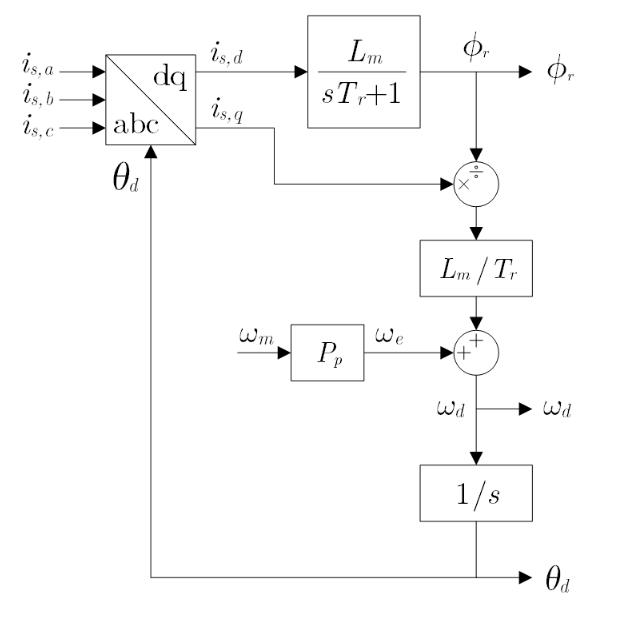
\includegraphics[width=0.5\linewidth]{IMAGES/Indus_el/Screenshot from 2025-04-14 16-56-04.png}
    \end{figure}
    \item DFOC : stator flux is determined through integration : $\phi_s = \int(v_s-R_s i_s)dt$. Then : $\phi_r = \frac{L_r}{L_m} (\phi_s - L_\sigma i_s)$.
    \begin{figure}[hbt!]
        \centering
        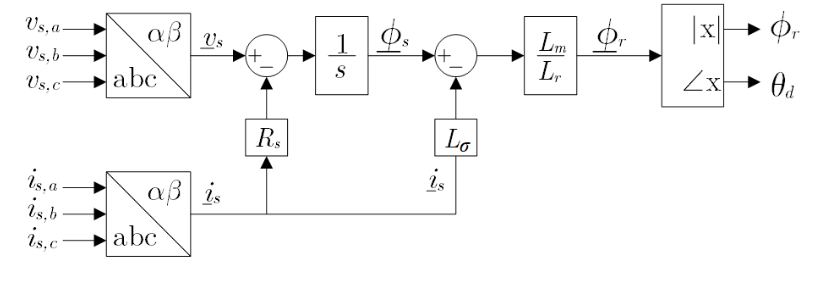
\includegraphics[width=0.5\linewidth]{IMAGES/Indus_el/Screenshot from 2025-04-14 17-02-59.png}
    
    \end{figure}
\end{itemize}

\subsubsection{Direct Torque Control}
Can be sensorless. It is done with space vector modulation. Let $S_a$, $S_b$, $S_c$ be the definition of each space vector : $\psi_{\alpha,\beta,s} = \frac{2}{3} V_{dc} (S_a + \alpha S_b + \alpha^2 S_c)t-R_s \int I_{\alpha,\beta,s} dt$. \\
\warning DC link voltage has influence on space vectors. It moves in the direction of the inverter space vector. It moves at constant angular speed, proportional to the output voltage. Compared to SVPWM sectors, there new sectors are shifted by $30^\circ$. \\

For flux control : \\
We want to control stator flux magnitude to be within some bounds around reference : $\lvert \phi_{\alpha,\beta,s}\rvert^*-\Delta \lvert \phi_{\alpha,\beta,s}\rvert/2 \leq\lvert \phi_{\alpha,\beta,s}\rvert \leq \lvert \phi_{\alpha,\beta,s}\rvert^* + \Delta \lvert \phi_{\alpha,\beta,s}\rvert/2$.\\
Magnitude error can be both positive and negative. \\

For torque control : \\
The torque can be controlled by the rate of change of the stator flux space vector. When actual torque is lower than desired torque : we should apply space vector that results in the fastest rate of change of $\omega_0$, this will result in the fastest change of torque. When actual torque is higher than desired one : it is better to decrease torque slowly, this will reduce switching frequency, zero space vectors are good choice.\\

If stator rotates clockwise, $T_{em}^* -\Delta T \leq T_{em} \leq T_{em}^*$. If stator rotates counter-clockwise : $T_{em}^* \leq T_{em} \leq T_{em}^*+\Delta T$.\\
\begin{figure}
    \centering
    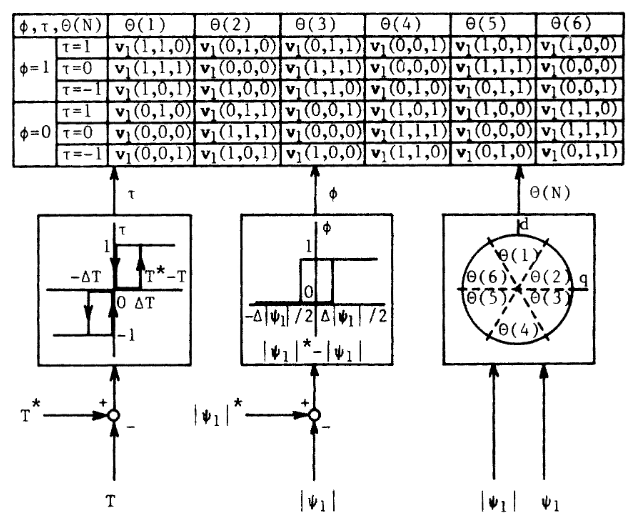
\includegraphics[width=0.5\linewidth]{IMAGES/Indus_el/Screenshot from 2025-04-28 16-54-53.png}
    \caption{Switching table.}
\end{figure}






TP3 : 
1) Vector control (or field-oriented control, FOC) offers superior performance compared to $U/f$ and direct torque control (DTC) by decoupling torque and flux control, enabling precise and dynamic control of induction machines. Unlike $U/f$ control, which can be open-loop and has limited dynamic response, vector control provides fast torque response and better efficiency. Compared to DTC, it generates less torque ripple and is more suitable for high-performance applications. A typical application where vector control excels is in electric vehicle drives, where fast torque response and efficiency are critical. However, it may not be ideal for simple applications like HVAC fans or pumps, where cost and simplicity outweigh performance requirements.

2)
Indirect Field-Oriented Control (IFOC) is a vector control technique used to control induction machines by decoupling the torque and flux-producing components of the stator current. The machine's dynamic equations are transformed into a synchronously rotating $(d,q)$ reference frame using the Park transformation. In this frame, the rotor flux is aligned with the $d$-axis, ensuring that the $q$-axis component of the rotor flux $\phi_{rq}$ is zero. As a result, the electromagnetic torque can be expressed as: $T_e = \frac{3}{2} \cdot \frac{P}{2} \cdot \frac{L_m}{L_r} \phi_r i_{sq}$. 
This decouples the control of torque (via $i_{sq}$) and rotor flux (via $i_{sd}$), making the system behave similarly to a separately excited DC motor.
Since rotor flux is not directly measurable, it is oriented indirectly by estimating the slip frequency: $\omega_{\text{slip}} = \frac{L_m}{T_r \phi_r} i_{sq}, \quad \text{with} \quad T_r = \frac{L_r}{R_r}$. Then $\omega_d = \omega_e + \frac{L_m}{T_r} \frac{i_{s,q}}{\phi_{r,d}}$ and $\frac{d\phi_{r,q}}{dt} + \frac{1}{T_r} \phi_{r,q} = 0$. The d-axis component is then : $\frac{d\phi_{r,d}}{dt} + \frac{1}{T_r} \phi_{r,d} = \frac{L_m}{T_r} i_{s,d}$.

PI controllers are typically used to regulate the $i_{sd}$ and $i_{sq}$ components of the stator current, and the resulting voltage commands are transformed back to the stationary reference frame for inverter control. This control strategy enables precise, dynamic torque and flux control, similar to that of a DC machine.


DFOC : 
Direct Field-Oriented Control (DFOC) is a vector control technique for induction machines that directly estimates and aligns the rotor flux with the $d$-axis of a synchronously rotating reference frame. Unlike Indirect Field-Oriented Control (IFOC), which relies on model-based slip calculation, DFOC uses real-time flux estimation methods based on measured stator voltages and currents.
By aligning the rotor flux vector along the $d$-axis ($\phi_{rq} = 0$), the torque can be controlled solely by the $q$-axis stator current component, and the flux by the $d$-axis component: $T_e = \frac{3}{2} \cdot \frac{P}{2} \cdot \frac{L_m}{L_r} \phi_r i_{sq}$.

To estimate the rotor angular frequency $\omega_r$ without deriving the angular position, one can calculate the slip frequency as: $\omega_{\text{slip}} = \frac{L_m}{T_r \phi_r} i_{sq}, \quad \text{where} \quad T_r = \frac{L_r}{R_r}$.
Then, using the known synchronous frequency $\omega_s$ from the controller, the rotor angular frequency is given by: $\omega_r = \omega_s - \omega_{\text{slip}}$.
This allows sensorless estimation of rotor speed without requiring the mechanical angular position.



\end{document}